\chapter{Simulation and Result Analysis}
\label{chap:Simulation_And_Result_Analysis}
This chapter shows and analyses the simulation results for four state estimation algorithms. Firstly, the performance over time is studied. Secondly, the influence of the location of the smart meters on the estimation accuracy is investigated and the optimal smart meters location is suggested. After that, the performance of the four estimators based on the proposed optimal smart meters location is compared to the cases with random smart meters location. Finally, the advantages and disadvantages of these four estimators are given.
\section{Performance Indices}
Before the result analysis, some performance indices are introduced in this section for determining the performance of the state estimation algorithms. 
\subsection{Absolute p.u. Error}
The most straightforward performance index is the absolute p.u. error between the estimated value and its real value without noise. All types of estimated measurements value can be obtained from the estimated state from the estimator together with the ideal measurement function $h_{ideal}(x)$. Compare to the measurement function $h(x)$ which calculates only the estimated value of the measurement from smart meters, $h_{ideal}(x)$ calculates the voltage magnitude, the power injection at all buses, and power flow on all branches of the system in p.u., which is shown below:
    \begin{align}
        h_{ideal}(x)=\begin{bmatrix}
                    V_e &
                    P_{inj-e} &
                    Q_{inj-e} &
                    P_{flow-e} &
                    Q_{flow-e} &
              \end{bmatrix}^\intercal
        \label{eq:ideal measurement jacobian  matrix}  
    \end{align}
, where $V_e$, $P_{inj-e}$ and $Q_{inj-e}$ represents the estimated voltage magnitude, active and reactive power injection at all buses in the system in p.u.. $P_{flow-e}$ and $Q_{flow-e}$ correspond to the active and reactive power flow over all branches in p.u..
The real value of the corresponding elements without noise in $h_{ideal}$ is called $z_{ideal}$, and the elements inside $z_{ideal}$ are shown in the equation below in p.u.:
    \begin{align}
        z_{ideal}=\begin{bmatrix}
                    V_{ideal} &
                    P_{ideal} &
                    Q_{ideal} &
                    P_{ideal} &
                    Q_{ideal} &
              \end{bmatrix}^\intercal
        \label{eq:ideal measurement}  
    \end{align}
Then, the absolute p.u. error can be calculated by using the estimated value $h_{ideal}$ minus its real value $z_{ideal}$. For example, the absolute voltage magnitude error $V_{error}^{i,t}$ of bus $i$ at time step $t$ in p.u. can be calculated as:
\begin{align}
    V_{error}^{i,t} &= |V_e^{i,t}-V_{ideal}^{i,t}|
    \label{eq:Verror}
\end{align}
All of the absolute p.u. errors are listed in Table \ref{tab:Error Types in p.u.}. The estimated and real value of the voltage phase angle is not included in $z_{ideal}$ or $h_{ideal}$.
    \begin{table}[!h]
        \centering
        \begin{tabular}{c|c|c}
            type of error & symbol & unit\\ \hline
            voltage magnitude & V_{error} & p.u. \\
            voltage phase angle & \theta_{error} & radian \\
            active power injection & P_{inj-error} & p.u. \\
            reactive power injection & Q_{inj-error} & p.u. \\
            active power flow & P_{flow-error} & p.u. \\
            reactive power flow & Q_{flow-error} & p.u. \\
        \end{tabular}
        \caption{Error Types in p.u.}
        \label{tab:Error Types in p.u.}
    \end{table}
\subsection{Ideal Cost}
The next performance index is a revised version of the cost function $J$ which can be called ideal cost function $J_{ideal}$ and calculated as follows:
\begin{align}
    J_{ideal}^t(x^t) &= (h_{ideal}(x^t)-z_{ideal}^t)^{\intercal} (h_{ideal}(x^t)-z_{ideal}^t)
    \label{eq:J_ideal}
\end{align}
, where $J_{ideal}^t(x^t)$ is the ideal cost under the state $x^t$ at time step t. Because there are totally 96 time steps in each case, then $t$ is ranging between 1 to 96 in this thesis. Compared to the cost function $J$, the ideal cost $J_{ideal}$ considering all error between estimated value and real value whereas cost $J$ only considering the error between estimated value and its corresponding measurement from smart meters with noise. 

\subsection{Root Mean Squared Error}
Root Mean Squared Error (RMSE) calculates the quadratic mean error between the prediction value and observed value over a certain time series. Because there is a square on the error ahead of the mean, RMSE is more sensitive to large error. In this project, the RMSE for each measurement in $z_{ideal}$ is calculated as follows:
\begin{align}
    RMSE &= \sqrt{ \frac{ \sum_{t=1}^{T} (\hat{y}^t-y^t) ^2}{T}}
    \label{eq:RMSE}
\end{align}
, where $\hat{y}^t$ is the predicted value at time step $t$ which can be replaced by the elements in $h_{ideal}(x^t)$ and $y^t$ is the real value which can be replaced by the corresponding value in $z^t_{ideal}$.

\subsection{Pearson Correlation Coefficient}
The Pearson correlation factor is a statistic factor which detects the linear relation between two variables and is denoted by $r$. The Pearson correlation factor takes values between -1 and 1. When $r$ is zero, it means that there is no correlation between these two variables. Negative $r$ indicates a negative correlation and a positive value means that there is a positive correlation between the two variables. The closer the absolute value of $r$ to 1, the stronger linear relation they have as shown in Figure \ref{fig:pearson_factor}:
    \begin{figure}[!h]
        \centering
        \includegraphics[ height=7cm, width=12cm]{figures/pearson.pdf}
        \caption{Different levels of Pearson correlation factor between two variables \cite{standard}}
        \label{fig:pearson_factor}
    \end{figure}
    
\noindent
The Pearson correlation coefficient $r$ between $X=[x_1,x_2,\cdots,x_n]$ and $Y=[y_1,y_2,\cdots,y_n]$ can be calculated by the equation below:
\begin{align}
    r &= \frac{\sum_{i=1}^{n}(x_i-\bar{x})(y_i-\bar{y})}{\sqrt{\sum_{i=1}^{n}(x_i-\bar{x})^2}\sqrt{\sum_{i=1}^{n}(y_i-\bar{y})^2}}
    \label{eq:pearson}
\end{align}
, where $\bar{x}$ is the mean value of $X$ and $\bar{y}$ is the mean value of $Y$. 

\subsection{Spearman Rank Correlation Coefficient}
\label{sect:spearman}
Spearman's rank correlation coefficient is used for detecting the positive or negative trend relation between two variables. Different from the Pearson correlation coefficient, the Spearman rank correlation coefficient does not require a constantly increasing or decreasing rate. The Spearman coefficient is close to 1 or -1 as long as the tested two variables are changing monotonically. So, the Spearman correlation coefficient can be understood as a Pearson correlated coefficient of ranked variables which gives the respondent a set of items and asks them to put the items in some form of order. Figure \ref{fig:spearman_factor} shows a clear view of the comparison between Pearson and Spearman correlation coefficients under different situations. 
    \begin{figure}[!h]
        \centering
        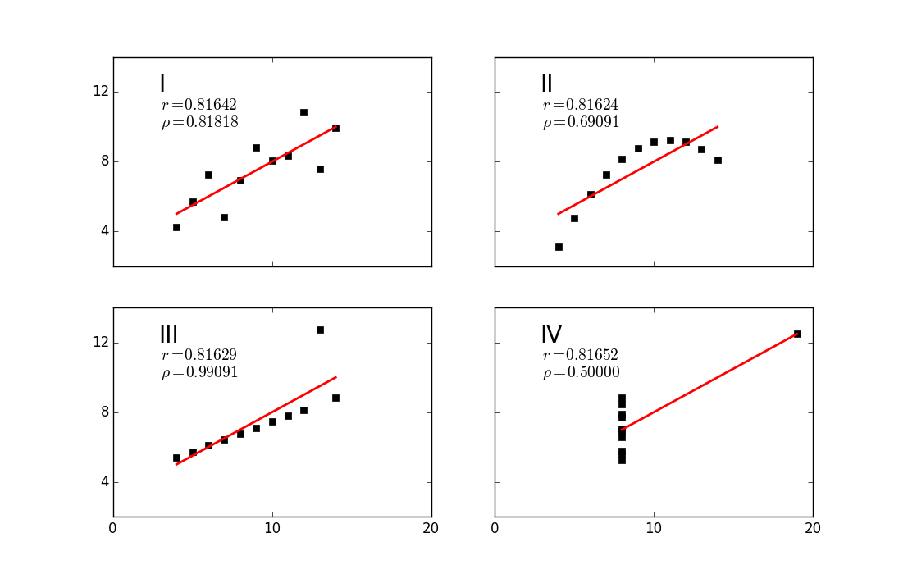
\includegraphics[ height=7cm, width=12cm]{figures/spearman.pdf}
        \caption{Comparison between Spearman and Pearson coefficient\cite{spearman}}
        \label{fig:spearman_factor}
    \end{figure}
By knowing the rank order of two variables, the Spearman correlated coefficient $\rho$ can be calculated as:
\begin{align}
    \rho &= 1- \frac{6 \sum_{i=1}^{n}d_i^2}{n(n^2-1)}
    \label{eq:spearman factor}
\end{align}
, where $d_i$ is the rank order difference at the $i^{th}$ observation and $n$ is the total number of observations. Because the Spearman correlation coefficient shows the rank order correlation, this factor is mainly used for detecting the influence of smart meters location on the accuracy of estimators, because the Pearson correlation coefficient shows the linear relationship between two variables whereas the trend of the correlation is more interested. Also, the index, which represents the smart meters distribution or distance, only shows the overall tendency of the smart meters location which makes Spearman correlation coefficient a more suitable index than Pearson correlation coefficient. 

\subsection{Standards for Correlation Coefficients}
\label{sect:threshold_0.3}
After obtaining the value of the correlation coefficients, it is necessary to build standards for determining the strength of the correlation between variables. Table \ref{tab:Correlation coefficient strength} shows a rough standard for determining the strength of the correlation factor. In this project, 0.3 is selected to be the threshold above which two variables are correlated.
    \begin{table}[!h]
        \centering
        \begin{tabular}{c|c}
            Absolute value & strengh\\ \hline
            .00 $\sim$ .19 &  $very \, weak(vw)$   \\
            .20 $\sim$ .39 &  $weak(w)$ \\
            .40 $\sim$ .59 & $moderate(m)$ \\
            .60 $\sim$ .79 & $strong(s)$ \\
            .80 $\sim$ 1.0 & $very \, strong(vs)$ \\
        \end{tabular}
        \caption{Correlation coefficient strength \cite{spearman_strength}}
        \label{tab:Correlation coefficient strength}
    \end{table}


\section{Result Analysis Over Time}
This section focuses on analyzing the error of the four estimators over time. For each scenario with different levels of measurements, there are 100 cases with different random location of smart meters. For each case, there are 96 time steps, which represents one day. After running the state estimation on 30 scenarios, the ideal cost $J_{ideal}^t$ is calculated by Equation \ref{eq:J_ideal} for each time step in each of the 100 cases and in each scenario. After that, the outliers of $J_{ideal}^t$ within 96 time steps in each case should be detected by using the 'isoutlier' function in MATLAB. The function 'isoutlier' calculates the median value of $J_{ideal}^t$ over the 96 time steps and the outliers in this function are defined as the value which is more than three scaled Median Absolute Deviations ($MADs$) the median value. For time series $X=[x_1,x_2,\cdots,x_n]$, the $MAD$ value can be derived as:
\begin{align}
    MAD &= med(|x_i-med(X)|)
    \label{eq:MAD}
\end{align}
, where $med$ means the median value of an array. In this case, only the values which exceed the upper threshold are defined as outliers, as shown in Figure \ref{fig:J ideal outlier}.
    \begin{figure}[!h]
        \centering
        \includegraphics[ height=7cm, width=12cm]{figures/J_ideal_outlier.pdf}
        \caption{J ideal outlier detection}
        \label{fig:J ideal outlier}
    \end{figure}
\bigskip
\\Table 4.3 summarizes the proportion of the error in voltage magnitude, active and reactive power injection, and active and reactive power flows in scenario 9. It comes out that the active power flows are responsible for a large portion of the error (i.e., $91 \%$ in scenario 9).
    \begin{table}[!h]
        \centering
        \begin{tabular}{c|c}
            type of error & proportion\\ \hline
            V_{error} &  {< 1 \%}   \\
            P_{inj-error} &  4 \% \\
            Q_{inj-error} & {< 1 \%} \\
            P_{flow-error} & 91 \% \\
            Q_{flow-error} & 4 \% \\
        \end{tabular}
        \caption{Proportion of each type of error in scenario 9}
        \label{tab:pie table}
    \end{table}
 The reason that the contribution from reactive power flow is smaller than that from active power flow is mainly because of the small constant power factor 0.98, and the reactive power consumption of each load is also relatively small compared with the active power consumption. Also, the number of branch power flow measurements is much higher than the other measurements due to the fact that there are two branch flow measurements (i.e., in both directions).
\bigskip
\\By knowing that most of the $J_{ideal}$ outliers are due to the high active power flow mismatch between the estimated value and real value, the next step is to find the reason of high active power flow mismatch at those time steps. Firstly, the number of times for $J_{ideal}$ to be an outlier at one time step in 100 cases for each scenario is figured out. Secondly, the next goal is to identify at which time step $J_{ideal}$ tends to be an outlier. 
\bigskip
\\Figure \ref{fig:outlier number} shows an example of the total number of outlier $J_{ideal}$ at each time step across 100 cases in scenario 9. The left y-axis is the number of outlier $J_{ideal}$ and the right y-axis shows the sum of the squared active power flow mismatchs between the real value without noise and the estimated value from WLS for 100 cases in scenario 9. As shown in table \ref{tab:pie table}, a large proportion of $J_{ideal}$ comes from the active power flow. Notice, notably, the correlation between the number of outlier $J_ideal$ per time step and the squared active power flow mismatch.
    \begin{figure}[!h]
        \centering
        \includegraphics[ height=9cm, width=14cm]{figures/outlier.pdf}
        \caption{Frequency of $J_{ideal}$ outliers together with the squared $P_{flow}$ mismatch across one day}
        \label{fig:outlier number}
    \end{figure}
The total active power injection at those time steps where $J_{ideal}$ is high is due to houseloads daily activities, which increases the power consumption and thus the active power flow at those time steps. As the pseudo-measurement generation method can not predict the active power injection well when the active power injection is relatively high and spiky, the mismatch between pseudo active power injection and its real value is large, which leads to high active power flow mismatch. To prove this assumption, the Pearson's correlation coefficient factor between the number of $J_{ideal}$ outliers and the mean value of the sum active power injection mismatch at each time step among the 100 cases is calculated for each of the 30 scenarios.The result for WLS is shown in Figure \ref{fig:pearson_J_ideal_30_scenario}. Notice that similar results are obtained with the other algorithms.
\bigskip
\\In the Figure \ref{fig:pearson_J_ideal_30_scenario}, the bottom x-axis shows the index of 30 scenarios and the top x-axis shows the measurements level for bus meters.
\begin{figure}[!h]
        \centering
        \includegraphics[ height=9cm, width=14cm]{figures/Pearson_J_ideal_outlier_WLS_bar.pdf}
        \caption{Pearson coefficient of active power injection mismatch and number of $J_{ideal}$ outliers for 30 scenarios}
        \label{fig:pearson_J_ideal_30_scenario}
\end{figure}
 For example, scenarios 3 to 5 represent the cases where $33\% $ of the buses have information of active power injection only, except the virtual measurements. And the blue, yellow and red bars correspond to the percentage of measured power flows, which are $0 \%$, $10 \%$, and $20 \%$, respectively. Except the case with $100 \%$ knowledge at buses, the correlation is relatively high and increases with the level of measurement penetration. However, scenarios 22 to 30 show a low correlation. This is mainly because there is no pseudo-measurements for active power injection anymore in these scenarios since the percentage of the buses which have information of active power injection is $ 100\% $ as shown in Table \ref{tab:30_scenarios}. Scenario 29 and 30 have a high Pearson factor compared with the other scenarios from 22 to 28 which does not fit the assumption that the active power injection mismatch does not have an influence on $J_{ideal}$ when the strong information of active power injection of all buses are known.
    \begin{figure}[!h]
        \centering
        \includegraphics[ height=7cm, width=12cm]{figures/max_num_of_times_J_ideal_outlier.pdf}
        \caption{Max $J_{ideal}$ outlier for each scenario}
        \label{fig:max_num_of_times_J_ideal_outlier}
    \end{figure}
The reason is mainly because the maximum number of times for $J_{ideal}$ to be an outlier across 96 time steps are relatively small in scenarios 29 and 30, as shown in Figure \ref{fig:max_num_of_times_J_ideal_outlier}.
\bigskip
\\In conclusion, a high mismatch between pseudo and real active power injection measurements leads to a high error on active power flows, which is the most important factor in $J_{ideal}$ as indicated in Table \ref{tab:pie table}. By neglecting the first three scenarios where all of the active power injections are pseudo measurements and last 9 scenarios where all of the buses have meters for measuring active power injection, the mean Pearson correlation coefficient between the active power injection mismatch and the number of $J_{ideal}$ outliers is shown in Table \ref{tab:pearson_J_ideal} four the four estimators. It can be seen that the mean value of the coefficients are close to 0.6 which show a moderately strong relationship between these two variables.
    \begin{table}[!h]
        \centering
        \begin{tabular}{c|c|c|c|c}
             & WLS & EKF & SHGM & SVR-EKF\\ \hline
            $r(num_{J_{ideal}},P_{mis-inj})$ & 0.6358($s$) & 0.6058($s$) & 0.6279($s$) &  0.5942($m$)\\
        \end{tabular}
        \caption{Mean Pearson coefficient of active power injection mismatch and number of $J_{ideal}$ outliers}
        \label{tab:pearson_J_ideal}
    \end{table}
    


\section{Influence of Smart Meter Location}
\label{sec:analysis_meter_location}
The section investigates the influence of smart meter location on the accuracy of the estimators. The bus meters are the smart meters measuring the voltage magnitude, active power injection, and reactive power injection. The branch meters are sensors measuring active and reactive power flows on the branches. With a given number of bus meters and branch meters, the accuracy of the estimation results is different according to their location. To simplify the problem, the interaction between the bus meters and branch meters is neglected, which means that the influence of the bus and branch meters location on the estimator accuracy is considered independently. 
\subsection{Hierarchy of Bus and Branch}
This section introduces a method for classifying the buses and branches in the radial network into different hierarchies based on the distance from the bus or branch meters to the feeder bus or branch. 
\bigskip
\\The radial network has a tree structure without closed loop.
    \begin{figure}[!h]
        \centering
        \includegraphics[ height=10cm, width=13cm]{figures/raidal_network_hierarchy.pdf}
        \caption{Hierarchy of buses and branches}
        \label{fig:radial hierarchy}
    \end{figure}
Figure \ref{fig:radial hierarchy} shows a simplified radial distribution grid with 13 buses, including the feeder bus at the top which is marked with 1. The hierarchy of a bus is defined as the distance from that bus to the feeder bus by assuming that the distance between two connected buses is one. In Figure \ref{fig:radial hierarchy} there are totally 4 layers in the bus hierarchy. The hierarchy of the feeder bus is defined as 1 and the hierarchy of the buses connected with feeder bus is 2, and so on. Since there is no closed loop, the distance between two buses, connected to a common upper hierarchy bus, is 2 as shown in Figure \ref{fig:distance_two_buses}.
    \begin{figure}[!h]
        \centering
        \includegraphics{figures/distance_two_buses.pdf}
        \caption{The distance between two neighbor buses}
        \label{fig:distance_two_buses}
    \end{figure}
\bigskip
\\The hierarchy of branches is similar to the hierarchy of buses. The branch, which connects feeder bus and buses in the first hierarchy, is defined as the branch in the first hierarchy, and the branch which connects buses in the $(n-1)^{th}$ hierarchy and buses in the $n^{th}$ hierarchy belongs to the $(n-1)^{th}$ branches hierarchy as shown in Figure \ref{fig:radial hierarchy}. But the fact that there is one thing different between the buses and branches is the buses which connect to the same bus at an upper hierarchy are not connected together as introduced in the last paragraph. But all the branches connected to one bus are assumed to connect together, which means in this case the distance between two branches connected to the same bus is 1. After defining the hierarchy index of buses and branches, the hierarchy of each bus or branch should be found by using Breadth-First search(BFS) algorithm which is widely used for searching tree or graph structure system.

\subsection{Path of Radial Network}
After giving the definition of the hierarchy of the buses and branches in the radial network, the concept of the path in a radial network should be introduced. In this project, the paths in the radial network are defined as a group of connected buses and branches, which go from the feeder bus to a "leaf" bus.
    \begin{figure}[!h]
        \centering
        \includegraphics[ height=8cm, width=12cm]{figures/path_radial_network.pdf}
        \caption{One path in radial network}
        \label{fig:path_radial_network}
    \end{figure}
Figure \ref{fig:path_radial_network} is a schematic diagram showing one of the seven paths in the radial network which is marked by a red line. The whole process is similar to the BFS except that the path search is from the bottom to the top and only the buses at higher hierarchy are searched. The pseudo code for finding the paths $Path$ is shown in the Appendix 5.3. 


\subsection{Influence of Smart Meters Distance to the Feeder Bus}
This section investigates the influence of the distance of meters to the feeder bus on the accuracy of estimators. The influence of bus meters and branch meters is investigated separately. Due to the fact that the voltage magnitudes and power flows are key quantities desired by DSO, only the accuracy of the bus voltage magnitudes and active and reactive power flows on the branches are considered as the criterion for the performance of estimators. The RMSE over 96 time steps is used as a metric. Taking the voltage magnitude as an example, one RMSE at each of the 206 buses, for each of the 30 scenarios and for each of the 100 corresponding cases is calculated. The mean $RMSE$ voltage magnitude across 206 buses for case $i$ in scenario $j$ is defined as follows:
\begin{align}
    RMSE^V_{i,j} &= \frac{1}{206} \sum_{k=1}^{206} RMSE_{i,j}(V^k)
    \label{eq:RMSE_V}
\end{align}
, where $RMSE^V_{i,j}$ represents the mean $RMSE$ value of the $i^{th}$ case in scenarios $j$ for all 206 buses in this thesis. $RMSE_{i,j}(V^k)$ indicates the voltage magnitude RMSE for the $k^{th}$ bus of the $i^{th}$ case in scenario $j$. Similarly, the active and reactive power flow error for the $i^{th}$ case in scenarios $j$ can be represented as $RMSE^{P_{flow}}_{i,j}$ and $RMSE^{Q_{flow}}_{i,j}$, respectively.
\bigskip
\\After showing the performance criteria for each case, the distance of the smart meters to the feeder bus can be defined. For instance, the distance from one bus meter at bus $v_i$ to the feeder bus $v_1$ is defined as:
\begin{align}
    dist_{i,j}(v_k) &= m^{v_k}_{i,j} ( hier(v_k) - hier(v_k) )
    \label{eq:dist_one_bus}
\end{align}
, where $dist_{i,j}(v_k)$ represents the distance from the smart meter at bus $v_k$ to the feeder bus $v_1$ of case $i$ in scenario $j$, and $m^{v_k}_{i,j}$ is a binary variable which indicates if there is a bus meter at bus $v_k$ of case $i$ in scenario $j$. $m^{v_k}_{i,j}$ equals to 1 if there is a bus meter at bus $v_k$ and equals to 0 if there is no meter at bus $v_k$. With the help of the hierarchy of each bus defined before, the distance from each bus meter to the feeder bus can be obtained easily. Then, the total distance $dist^{bus}_{i,j}$ from all bus meters to the feeder bus of the case $i$ in scenario $j$ can be calculated by:
\begin{align}
    dist^{bus}_{i,j} &= \sum_{k=1}^{206} dist_{i,j}(v_k)
    \label{eq:dist_bus}
\end{align}
And the branch meters distance to the feeder bus $dist^{branch}_{i,j}$ from all branch meters to the branches connected to the feeder bus of the case $i$ in scenario $j$ can be calculated in the same way. Nevertheless, notice that if there are two branch meters connected at the same branch, they are counted as one branch meter, because there is no significant influence on the accuracy of the estimator between one meter or two meters on the same branch.
\bigskip
\\After obtaining the bus and branch meter distances to the feeder bus for 100 cases in each scenario and the corresponding $RMSE_j^V$, $RMSE_j^{P_{flow}}$ and $RMSE_j^{Q_{flow}}$ which represents the $RMSE$ for 100 case in scenario $j$ for $j=1,2,\cdots,30$, where $RMSE_j^V=\{RMSE_{1,j}^V,RMSE_{2,j}^V,\cdots,RMSE_{100,j}^V \}$, $\{RMSE_{1,j}^{P_{flow}},RMSE_{2,j}^{P_{flow}},\cdots,RMSE_{100,j}^{P_{flow}} \}$, and $\{RMSE_{1,j}^{Q_{flow}},RMSE_{2,j}^{Q_{flow}},\cdots,RMSE_{100,j}^{Q_{flow}} \}$, the Spearman's correlation coefficient is used as explained before in Sect. \ref{sect:spearman}. Take the bus meters as an example, the Spearman's correlation coefficient $p(RMSE_j^V,dist_j^{bus})$ between the voltage magnitude $RMSE_j^V$ and distance of the bus meters to the feeder bus $dist_j^{bus}=\{dist_{1,j}^{bus},dist_{2,j}^{bus},\cdots,dist_{100,j}^{bus} \}$ in scenario $j$ can be calculated by Equation \ref{eq:spearman factor}. After calculating the Spearman's correlation coefficient $p(RMSE_j^V,dist_j^{bus})$ since $j=1,\cdots,30$, the mean Spearman correlation coefficient is defined as $p(RMSE^V,dist^{bus})$.
\bigskip
\\The process for detecting the Spearman's correlation coefficient between the distance of branch meters to the feeder bus and different types of error is the same as the one with bus meters. 
    
\subsubsection{Result of the Influence of Meter Distance to Feeder Bus}
    \begin{table}[!h]
        \centering
        \begin{tabular}{c|c|c|c|c}
             & WLS & EKF & SHGM & SVR-EKF\\ \hline
            $p(RMSE^V,dist^{bus})$ & 0.0821($vw$) & 0.0839($vw$) & 0.0816($vw$) &  0.1295($vw$)\\
            $p(RMSE^{P_{flow}},dist^{bus})$ & 0.0647($vw$) & 0.0667($vw$) & 0.0662($vw$) &  0.0582($vw$)\\
            $p(RMSE^{Q_{flow}},dist^{bus})$ & 0.0915($vw$) & 0.0937($vw$) & 0.0846($vw$) &  0.0797($vw$)\\
            $p(RMSE^V,dist^{branch})$ & 0.1521($vw$) & 0.1404($vw$) & 0.0848($vw$) &  0.1539($vw$)\\
            $p(RMSE^{P_{flow}},dist^{branch})$ & 0.1003($vw$) & 0.0936($vw$) & 0.1120($vw$) &  0.1473($vw$)\\
            $p(RMSE^{Q_{flow}},dist^{branch})$ & 0.1074($vw$) & 0.0963($vw$) & 0.1025($vw$) &  0.1288($vw$)\\
        \end{tabular}
        \caption{Mean Spearman coefficient of meter distance to feeder bus and RMSE}
        \label{tab:spearman_meter_dist}
    \end{table}
\noindent    
Table \ref{tab:spearman_meter_dist} shows the mean value of the Spearman's correlation coefficient across 30 scenarios between bus or branch meters distance to the feeder bus and the error in the estimation of voltages, active and reactive power flows. The details of the Spearman coefficient value can be found in Appendix A.1. It can be seen from the table that the correlation is very weak in all cases. Hence, it can be concluded that the distances of bus or branch meters to the feeder bus have no influence on the accuracy of estimated voltage magnitude, active power flow, and reactive power flow for these four estimators.

\subsection{Influence of Smart Meters Distribution}
This section investigates the influence of the distribution of bus meters and branch meters on the accuracy of estimators. 
\subsubsection{Definition of Meter Distribution}
The aim of this section is to define how to identify if bus meters or branch meters are well distributed or not. For instance, the $dist_{i,j}^{close}{ ( v_k ) }$ corresponds to the distance from bus $v_k$ to the closest bus with a meter for case $i$ in scenario $j$. Once all $dist_{i,j}^{close}{ ( v_k ) }$ for all of the buses are calculated, they are summed together and the total distribution factor $distr^{bus}_{i,j}$ for the bus meters at the $i^{th}$ case in scenario $j$ can be obtained:
\begin{align}
    distr^{bus}_{i,j} &= \sum_{k=1}^{206} dist_{i,j}^{close}{(v_k)}
    \label{eq:distr_bus}
\end{align}
And the distribution factor $distr^{branch}_{i,j}$ of branch meters in case $i$ of scenario $j$ can be obtained with the same method by summing the distance from each branch $e_i$ to the closest branch with a meter:
\begin{align}
    distr^{branch}_{i,j} &= \sum_{k=1}^{205} dist_{i,j}^{close}{(e_k)}
    \label{eq:distr_branch}
\end{align}
If the value of $distr^{bus}_{i,j}$ is small, it means that there is a bus meter close to each bus and the bus meters are well distributed acorss the system. On the contrary, the bus meters are not well distributed when $distr^{bus}_i$ is larger, meaning that meters are mainly concentrated at a few buses.

\subsubsection{Searching the Closest Meter by BFS}
\label{sect:BFS_dist}
Before calculating the distribution factor $distr$, it is necessary to get the distance $dist_{i,j}^{close}{ ( v_k ) }$ from each bus $v_k$ to its closest meter for $k=1,\cdots,206$ in the $i^{th}$ case of the $j^{th}$ scenario. There are two definitions for the closest metered bus to each bus, through Breath-First Search (BFS) or Path Search.
    \begin{figure}[!h]
        \centering
        \includegraphics[ height=9cm, width=14cm]{figures/topo_new.pdf}
        \caption{Two method for obtaining $dist_{i,j}^{close}{ ( v_{red} ) }$}
        \label{fig:distr_topo}
    \end{figure} 
\bigskip
\\Figure \ref{fig:distr_topo} shows a simplified distribution grid with 13 buses where the blue buses have a meter and the red line shows the path connected with the red bus which is considered. By using BFS, the closest bus meter to the red bus is the blue one at the fourth hierarchy. So, $dist_{i,j}^{close}{(v_{red})}=2$ in this case based on BFS. Analogously, the distance $dist_{i,j}^{close}{(e_i)}$ from  to the branch $e_i$ to its closest branch meter can be obtained with the same method. The pseudo-code for the whole procedure can be found in Appendix 5.3.3.
\bigskip
\\After finding the distance from each bus or branch to their closest metered bus or branch, the distribution of bus meters $distr_{i,j}^{bus}$ and branch meters $distr_{i,j}^{branch}$ for case $i$ in scenario $j$ can be calculated by Equation \ref{eq:distr_bus}. And the Spearman's correlation coefficients between meter distribution and the different errors in consideration, for the four estimators and for each scenario can be obtained, whose details are shown in Appendix A.1. FOr instance, $p(RMSE_j^V,distr_j^{bus})$ represents the Spearman correlation coefficient between mean voltage magnitude error $RMSE_j^V=\{RMSE_{1,j}^V,RMSE_{2,j}^V,\cdots,RMSE_{100,j}^V \}$ and bus meters distribution $distr_j^{bus}=\{distr_{1,j}^{bus},distr_{2,j}^{bus},\cdots,distr_{100,j}^{bus} \}$ based on BFS in scenario $j$. After that, the mean Spearman's factor $p(RMSE_j^V,distr_j^{bus})$ for 30 scenarios and for  each estimator can be calculated. Similarly, the Spearman correlation coefficient for the other types of error and meters distribution based on BFS can be calculated, and their values are listed in Table \ref{tab:spearman_meter_distr_BFS}. It can be seen that all the mean Spearman's correlation coefficients show a very weak correlation, well below the threshold 0.3. As a result, the conclusion can be drawn that the distribution of bus meters and branch meters based on BFS does not influence the voltage magnitude error $RMSE^V$, active power flow error $RMSE^{P_{flow}}$, and reactive power flow error $RMSE^{Q_{flow}}$ for the four state estimation algorithms.

    \begin{table}[!h]
        \centering
        \begin{tabular}{c|c|c|c|c}
             & WLS & EKF & SHGM & SVR-EKF\\ \hline
            $p(RMSE^V,distr^{bus})$ & 0.0664($vw$) & 0.0609($vw$) & 0.0584($vw$) &  0.0847($vw$)\\
            $p(RMSE^{P_{flow}},distr^{bus})$ & 0.0916($vw$) & 0.0900($vw$) & 0.0942($vw$) &  0.1073($vw$)\\
            $p(RMSE^{Q_{flow}},distr^{bus})$ & 0.0917($vw$) & 0.0970($vw$) & 0.0919($vw$) &  0.0843($vw$)\\
            $p(RMSE^V,distr^{branch})$ & 0.0964($vw$) & 0.0955($vw$) & 0.0766($vw$) &  0.1143($vw$)\\
            $p(RMSE^{P_{flow}},distr^{branch})$ & 0.2759($w$) & 0.2063($w$) & 0.2150($w$) &  0.1556($vw$)\\
            $p(RMSE^{Q_{flow}},distr^{branch})$ & 0.2755($w$) & 0.2325($w$) & 0.2493($w$) &  0.1694($vw$)\\
        \end{tabular}
        \caption{Mean Spearman Coefficient of Meter Distribution by BFS and RMSE}
        \label{tab:spearman_meter_distr_BFS}
    \end{table}


\subsubsection{Searching the Closest Meter by Path Search}
\label{sect:Path_dist}
Another definition of $dist_{i,j}^{close}{(v_i)}$ is searching the closest distance from bus $v_i$ to a metered bus only on the same path. For example in Figure \ref{fig:distr_topo}, the closest metered bus to the red bus is the blue one on the fourth hierarchy on the left whose $dist_{i,j}^{close}{(v_{red})}$ equals to 2 according to BFS. However, these two buses do not lie on the same path. The closest metered bus on the same path is the feeder bus at the first hierarchy whose distance $dist_{i,j}^{close}{(v_{red})}$ is 3. As a result, a different value of $dist_{i,j}^{close}{(v_i)}$ is obtained based on Path Searching and results in a different value of the total meter distribution value $distr_{i,j}^{bus}$ or $distr_{i,j}^{branch}$ for metered buses and branches in the $i^{th}$ case of scenario $j$, respectively. And the pseudo-code for searching the distance $dist_{i,j}^{close}{(v_{red})}$ from bus $v_{red}$ to its closest metered bus by Path Search for case $i$ in scenario $j$ is shown in Algorithm \ref{alg:searching meter PS}, where $M_{i,j}^{bus}= \{v_1,\cdots,v_m \}$ is the set of buses who have a metered bus in the $i^{th}$ case of scenario $j$, $p_i=(p_i^v,p_i^e)$ is the $i^{th}$ path, and $Path=(p1,\cdots,p_{np})$ includes all paths in system $G=(V,E)$.

\bigskip
\begin{algorithm}[H]
\KwData{G=(V,E), M_{i,j}^{bus}, Path=(p1,\cdots,p_{np}), p_i=(p_i^v,p_i^e)}
\KwResult{dist_{i,j}^{close}{(v_{red})}}
\Initialize{\textbf{Initialize:} $L=\{v_{red}\}$, $k=0$, $a=\infty$\;}

\eIf{$L$ \cap $M_{i,j}^{bus}$ \neq $\emptyset$}
{$dist_{i,j}^{close}{(v_{red})} = k$}
{$do \, nothing$}
\For{p_i \in Path}{
    \eIf{$v_{red}$ \in $p_i^v$}
    {
        $M^s = p_i^v \cap M_{i,j}^{bus}$\;
        \For{$m \in M^s$}{
            $b=|hier(m)-hier(v_{red})|$
            \eIf{$b<a$}{
                $dist_{i,j}^{close}{(v_{red})} = b$\;
            }{
                $do$ \, $nothing$
            }            
        }
        
    }
    {
        $do \, nothing$
    }
}
\caption{Searching $dist_{i,j}^{close}{(v_{red})}$ by Path Search}
\label{alg:searching meter PS}
\end{algorithm}

\bigskip
\noindent
\\Notice that there is always at least one bus meter installed at the feeder bus at the same path with $v_{red}$. However, there might be no metered branch connected on the same path as the branch $e_{red}$. As a result, when there is no metered branch along the path of branch $e_{red}$, the distance $hier(e_s)-hier(e_1)$ between feeder branch and its closest meter at branch $e_s$ must be added to $hier(e_{red})-hier(e_1)$ to get the distance from branch $e_{red}$ to its closest metered branch:
\begin{align}
    dist_{i,j}^{close} (e_{red}) &= hier(e_s)-hier(e_1) + hier(e_{red}) - hier(e_1)
    \label{eq:branch_meter_path}
\end{align}
After obtaining the $dist_{i,j}^{close}$ for all of the buses and branches for cases $i$ in scenario $j$, the distribution factor $distr$ for metered buses and branches can be calculated by Equation \ref{eq:distr_bus} and \ref{eq:distr_branch}. Then, the Spearman's correlation coefficient between bus or branch meters distribution and error can be calculated for each scenario, which is shown in Appendix A.1. By calculating the mean value of Spearman's factor over 30 scenarios, Table \ref{tab:spearman_meter_distr_path} can be obtained.
    \begin{table}[!h]
        \centering
        \begin{tabular}{c|c|c|c|c}
             & WLS & EKF & SHGM & SVR-EKF\\ \hline
            $p(RMSE^V,distr^{bus})$ & 0.0776($vw$) & 0.0904($vw$) & 0.0975($vw$) &  0.0858($vw$)\\
            $p(RMSE^{P_{flow}},distr^{bus})$ & 0.0982($vw$) & 0.1030($vw$) & 0.1031($vw$) &  0.0970($vw$)\\
            $p(RMSE^{Q_{flow}},distr^{bus})$ & 0.0991($vw$) & 0.1024($vw$) & 0.0938($vw$) &  0.0831($vw$)\\
            $p(RMSE^V,distr^{branch})$ & 0.2346($w$) & 0.2516($w$) & 0.0977($vw$) &  0.3823($w$)\\
            $p(RMSE^{P_{flow}},distr^{branch})$ & 0.3295($w$) & 0.2934($w$) & 0.3183($w$) &  0.4037($m$)\\
            $p(RMSE^{Q_{flow}},distr^{branch})$ & 0.3453($w$) & 0.2691($w$) & 0.3358($w$) &  0.3355($w$)\\
        \end{tabular}
        \caption{Mean Spearman Coefficient of Meter Distribution by path and RMSE}
        \label{tab:spearman_meter_distr_path}
    \end{table}
\bigskip
\\The first three rows in Table \ref{tab:spearman_meter_distr_path} show the mean Spearman's coefficient between the bus meter distribution and three types of errors. All of them show a very weak correlation between bus meters distribution and the $RMSE$ , well below 0.3. In addition, the distribution of the branch meters has no significant influence on the accuracy of the voltage error $RMSE^V$ where nearly all of the Spearman's factors are below but close to 0.3 except SVR-EKF. However, almost all of the Spearman's correlation coefficients between branch meters distribution and power flow errors are higher than 0.3 (except EKF). Hence, it can be concluded that the distribution of the branch meters based on Path Search influences the active power flow error $RMSE^{P_{flow}}$ and reactive power flow error $RMSE^{Q_{flow}}$. The better distributed the branch meters are, the lower the power flow error.

\subsubsection{Summary}
Based on the previous simulation results of meters distribution on the estimators' accuracy, it can be seen that the meter distribution method based on BFS has no influence on the mean $RMSE^V$, $RMSE^{P_{flow}}$, and $RMSE^{Q_{flow}}$. Also, the bus meters distribution based on Path Search has no influence on the mean $RMSE^V$, $RMSE^{P_{flow}}$, and $RMSE^{Q_{flow}}$ for the tested four estimators in the radial distribution grid. But $RMSE^{P_{flow}}$ and $RMSE^{Q_{flow}}$ can be reduced by properly distributing the branch meters based on the Path Search. Since the above errors can be reduced when $distr^{branch}$ is smaller, for a giving number of branch meters, it is better to install them as well distributed as possible based on the Path Search.

\subsection{Influence of Bus Meters Location based on Power Injection}
This section investigates the location bus meters for increasing the accuracy of the state estimation algorithms. The original idea is that the accuracy of the pseudo-measurements at different buses is different. If the given bus meters are installed at the buses whose potential pseudo-measurements are not accurate, then the pseudo-measurements with high mismatch can be avoided, and the performance of the estimators can be increased by increasing the accuracy of pseudo-measurements. As a result, the aim is to find the buses whose potential pseudo-measurements have low accuracy and install smart bus meters at these buses.

\subsubsection{Influence of Pseudo-Measurements Accuracy on State Estimation}
The first step is to detect if the accuracy of the pseudo-measurements has an influence on the performance of the state estimation algorithms. Assuming $p_{psu-inj}^i(t)$ is the $i^{th}$ pseudo active power injection measurement at time step $t$ and $p_{inj}^i(t)$ is its corresponding real value. Then, the total active power mismatch $mis^{P}$ for all pseudo active power injection and 96 time steps at this case is:
\begin{align}
    mis^{P} &= \sum_{i=1}^{m_p} \sum_{t=1}^{96} |p_{psu-inj}^i(t)-p_{inj}^i(t)|
    \label{eq:total_mismatch}
\end{align}
, where $m_p$ is the total number of pseudo active power injection measurements in the grid. The total reactive power mismatch $mis^{Q}$ for each case can be calculated in the same way. The Pearson correlation coefficient between active power mismatch and its corresponding mean voltage, active and reactive power flow error over 100 cases for each scenario can be derived, respectively. In this project, only the influence of the active power injection mismatch $mis^{P}$ is investigated because the power factor of the loads is assumed to be constant, which means that the changing tendency between active power injection and reactive power injection is nearly the same.
    \begin{table}[!h]
        \centering
        \begin{tabular}{c|c|c|c|c}
             & WLS & EKF & SHGM & SVR-EKF\\ \hline
            $r(RMSE^V,mis^{P})$ & 0.1959($vw$) & 0.1851($vw$) & 0.2212($w$) &  0.2528($w$)\\
            $r(RMSE^{P_{flow}},mis^{P})$ & 0.4883($m$) & 0.4975($m$) & 0.5878($m$) &  0.6418($s$)\\
            $r(RMSE^{Q_{flow}},mis^{P})$ & 0.3460($m$) & 0.3535($m$) & 0.3837($m$) &  0.4241($m$)\\
        \end{tabular}
        \caption{Mean Pearson Coefficient between active power injection mismatch and RMSE}
        \label{tab:pearson_mis_error}
    \end{table}
Table \ref{tab:pearson_mis_error} shows the mean Pearson's coefficients between the total active power injection mismatch and the error in state estimation over 30 scenarios. It can be seen that there is a overall moderate to strong relation between the total active power injection mismatch and both active and reactive power flow errors. The mean correlation with the voltage error is very week (i.e., lower than the defined threshold of 0.3). However, when looking at the result for each individual scenario, it appears that the voltage error is strongly correlated with the total mus injection mismatch whenever there a no power flow measurements but smart meters also provide information about the voltage (i.e., scenarios 10 and 19).
    \begin{figure}[!h]
        \centering
        \includegraphics[ height=9cm, width=14cm]{figures/mis_pinj_error.pdf}
        \caption{Pearson's coefficient $r(RMSE^V,mis^{P})$ for 30 scenarios}
        \label{fig:mis_Pinj_error}
    \end{figure} 
For SVR-EKF, $r(RMSE^V,mis^{P})$ is higher than the threshold of 0.3 as long as there is no power flow measurements. The correlation coefficients from scenario 1 to 3 are zero because all of the active power injections are pseudo measurements and $mis^{P}$ is therefore constant. Concerning scenarios 22 to 30 the active power injection for all the buses are measured such that there is no pseudo-measurements for active power injection.
\bigskip
\\To conclude, the accuracy of the pseudo-measurements for active power have an influence on the result of power flow. As for the voltage magnitude accuracy for WLS, EKF, and SHGM, it can only be influenced by the placement of smart meters whenever they provide voltage information. Finally, the voltage magnitude error in SVR-EKF is correlatied with the accuracy of the pseudo
active power injection only if there are no branch meters.

\subsubsection{Accuracy of Pseudo-Measurements}
After knowing that the accuracy of the pseudo active power injection has an effect on the accuracy of the estimators, it is important to investigate the methods for improving the accuracy of the pseudo-measurements. The idea is that nearly all the loads in this project are residential consumers, which means that their active power injection can be very volatile within one day. So, the hypothesis is made that the total mismatch between the pseudo active power injection and its corresponding real value at bus $i$ $P^{mis}_i$ for one day is high when the total active energy consumption $E_c^i$ at bus $i$ for one day is high. To prove this hypothesis, the Pearson's correlation coefficient $p(P^{mis},E_c)$ between the total active power injection mismatch $P^{mis}= \{ P^{mis}_1,P^{mis}_2,\cdots,P^{mis}_{206} \}$ and the total active energy consumption $E_c= \{E_c^1,E_c^2,\cdots,E_c^{206} \}$ for all buses within one day is calculated. After calculating $p(P^{mis},E_c)$ for 100 cases in 30 scenarios. The boxplot figure with 100 $p(P^{mis},E_c)$ in each of 30 scenarios is shown in Figure \ref{fig:p_tot_p_mis}. Notice that in scenarios 1 to 3, the active power injections at all 205 buses except the feeder bus are pseudo measurements such that there is no difference between the 100 cases from scenario 1 to 3. 
    \begin{figure}[!h]
        \centering
        \includegraphics[ height=8cm, width=14cm]{figures/p_tot_p_mis.pdf}
        \caption{100 Pearson's coefficient $p(P^{mis},E_c)$ for 30 scenarios}
        \label{fig:p_tot_p_mis}
    \end{figure}     
In scenarios 22 to 30, there is no pseudo active power injection we cannot compute the correlation. It can be seen that even the lowest $p(P^{mis},E_c)$ is still above 0.7, so the conclusion can be drawn that the accuracy of the pseudo active power injection is reduced when the total power injection at that bus is high.

\subsubsection{Suggested Location for Bus Meters}
By knowing that there is a strong relation between the total active energy consumption and accuracy of its corresponding pseudo active power injection, installing smart meters at the buses whose total active energy consumption is high, the overall accuracy of the pseudo active power injections can be increased. Indeed, the pseudo active power injections would need to be computed at the buses whose total active energy consumption is low, which leads to a higher accuracy on pseudo-measurements. As a result, the accuracy of the estimators can be increased as shown in Table \ref{tab:pearson_mis_error}. For this purpose, the Pearson's correlation coefficient between the active energy consumption  $E^{psu}$ at the buses with pseudo active power injection and the three types of errors $RMSE^{V}$, $RMSE^{P_{flow}}$ ,and $RMSE^{Q_{flow}}$ is calculated for each scenario. The active energy consumption at the buses with pseudo active power injection $E^{tot}$ is calculated by the Equation \ref{eq:E^{psu}}:
\begin{align}
    E^{psu} &= \sum_{i=1}^{m_p} E_c^{v_p^{i}}
    \label{eq:E^{psu}}
\end{align}
, where $E_c^{v_p^{i}}$ is the active energy consumption at bus $v_p^{i}$ which is the $i^{th}$ bus with pseudo active power injection, and $m_p$ is the total number of buses which needs a pseudo active power injection. Because the number of the bus meters is constant for all 100 cases in each scenario, a higher $E^{psu}$ corresponds to a higher mismatch between the pseudo active power injections and their real value , according to the $r(P^{mis},E_c)$ shown in Figure \ref{fig:p_tot_p_mis}.  The Pearson's correlation coefficient between  $E^{psu}$ and the three average errors $RMSE^{V}$, $RMSE^{P_{flow}}$ ,and $RMSE^{Q_{flow}}$ for all 30 scenarios can be found in Appendix A.2. The mean Pearson's correlation coefficient between $E^{psu}$ and these errors over 30 scenarios are shown in Table \ref{tab:pearson_p_tot_error}. 
    \begin{table}[!h]
        \centering
        \begin{tabular}{c|c|c|c|c}
             & WLS & EKF & SHGM & SVR-EKF\\ \hline
            $r(RMSE^V,E^{psu})$ & 0.1851($vw$) & 0.1677($vw$) & 0.1989($vw$) &  0.2825($w$)\\
            $r(RMSE^{P_{flow}},E^{psu})$ & 0.4556($m$) & 0.4651($m$) & 0.5575($m$) &  0.5974($m$)\\
            $r(RMSE^{Q_{flow}},E^{psu})$ & 0.4568($m$) & 0.4643($m$) & 0.5155($m$) &  0.5455($m$)\\
        \end{tabular}
        \caption{Mean Pearson Coefficient of Meter location between $E^{psu}$ and mean RMSE}
        \label{tab:pearson_p_tot_error}
    \end{table}
It can be found that the Pearson's coefficient $r(RMSE^{P_{flow}},E^{psu})$ and $r(RMSE^{Q_{flow}},E^{psu})$ for all of the four estimators are higher than the threshold of 0.3, which proves that the active and reactive power flow errors can be reduced when the bus meters are installed at the buses with high active energy consumption. Similarly, to $r(RMSE^V,mis^P)$, even though the mean value $r(RMSE^V,E^{psu})$ over 30 scenarios is smaller than 0.3 for all four estimators, there are some specific
scenarios where $r(RMSE^V,E^{psu})$ shows a stronger relation as shown in Figure \ref{fig:p_tot_error}.
    \begin{figure}[!h]
        \centering
        \includegraphics[ height=8cm, width=14cm]{figures/p_tot_error.pdf}
        \caption{Pearson's correlation coefficient between active energy consumption and total active power mismatch for 30 scenarios}
        \label{fig:p_tot_error}
    \end{figure}      
For WLS, EKF, and SHGM, the scenarios 10 and 19 show a moderate to strong relation between the active energy consumption for buses with pseudo measurements and the voltage error $RMSE^V$. Both of them have information for the voltage magnitude but no branch meters are installed. As for SVR-EKF, the Pearman's factor $r(RMSE^V,E^{psu})$ is higher than the threshold 0.3 as long as there is no information for power flows.
\bigskip
\\Based on the analysis above, the conclusion can be drawn that the mean active and reactive power flow error can be reduced by installing the bus meters at the buses whose active energy consumption is known to be generally high. In addition, this can reduce the mean voltage magnitude error when the information of voltage magnitude is also known at the smart meters. To conclude, if there are totally $m^{bus}$ number of bus meters available, the performance of the state estimator can theoretically be improved by installing them at the $m^{bus}$ buses with the highest overall active energy consumption .

\subsection{Testing the Smart Meter Installing Strategy}
Based on the investigation of the influence of the smart meter location on the performance of state estimation algorithms, the following two points can be concluded:
\begin{itemize}
    \item Bus Meter: Installing bus meters at the buses with the highest overall active energy consumption.

    \item Branch Meter: Installing branch meters as well distributed as possible based on the Path Search.
 
    
\end{itemize}
The bus meters installation method is straightforward since the total active energy consumption at all bus can be, in principle, known. As for the location of branch meters, because it is not straighforward to find the optimal case with the lowest value of $distr^{branch}$, the suggested optimal branch meters locations is picked out of the mentioned 100 cases in each of the 30 scenarios. When $10 \% $ of power flow information is known, the smallest $distr^{branch}$ is searched among the scenarios 2, 5, 8, 11, 14, 17, 20, 23, 26, and 29. The smallest $distr^{branch}$ with $20 \%$ of measured power flow is searched within scenarios 3, 6, 9, 12, 15, 18, 21, 24, 27, and 30.
\bigskip
\\After determining the suggested optimal smart meters installation for all 30 scenarios, four state estimation algorithms are run again for each scenario and their accuracy for $RMSE^V$, $RMSE^{P_{flow}}$, and $RMSE^{Q_{flow}}$ is compared with the previously mentioned 100 cases in each scenario.

\subsubsection{Voltage Magnitude Error}
Figure \ref{fig:compare_V} shows the comparison of the voltage error $RMSE^V$ comparison between the proposed optimal smart meter location method and 100 cases in each of 30 scenarios for four estimators. The y-axis is the percentage out of the 100 cases in each scenario which have a higher $RMSE^V$ than the the proposed optimal smart meters location.
    \begin{figure}[!h]
        \centering
        \includegraphics[ height=8cm, width=14cm]{figures/v.pdf}
        \caption{$RMSE^V$ comparison}
        \label{fig:compare_V}
    \end{figure}
The values for scenario 1, 22, 25, and 28 are zero because there is only one possible smart meters location. For WLS, EKF, and SHGM, the proposed smart meters location method can clearly reduce the $RMSE^V$ when the information of the voltage magnitudes is known as shown in scenario 10 and 19, where nearly all of the 100 cases exhibit a higher error than the optimal smart meters location. But the optimality of the smart meters location is not as strong when the level of actual measurements increases. For example, the percentage decreases from scenario 10 to 12 when more branch meters are installed, as well as in the scenarios 23 to 30. As for the SVR-EKF, the mean voltage error is smaller based on the optimal smart meter location method as long as the level of measurements is small. 
\bigskip
\\To conclude, the voltage error can clearly be reduced by using the proposed optimal smart meter location method when the information of voltage magnitudes is known and the level of power flow measurements is low for WLS, EKF, and SHGM. As for SVR-EKF, the performance of the proposed optimal smart meter location selection method slightly decreases when the level of power flow measurements increases.

\subsubsection{Active Power Flow Error}
Figure \ref{fig:compare_P} compares the active power flow error $RMSE^{P_{flow}}$ of the simulation with the optimal smart meters location method with the other 100 cases for each scenario.
    \begin{figure}[!h]
        \centering
        \includegraphics[ height=8cm, width=14cm]{figures/pflow.pdf}
        \caption{$RMSE^{P_{flow}}$ comparison}
        \label{fig:compare_P}
    \end{figure}
For WLS and SHGM, it can be seen that nearly all of the 100 cases show a higher active power flow error than the optimal smart meter location method. But the percentage of 100 cases with a higher $RMSE^{P_{flow}}$ is slightly reduced in scenarios 3, 24, 27, and 30. Scenario 3 shows similar characteristics for all of 4 estimators with a slightly lower percentage. Scenarios 24, 27 and 30 are characterized by a full knowledge of the active power injection and $20 \%$ of power flows measurements. In such conditions, the suggested optimal meter location clearly fails for EKF based algorithms.
    \begin{figure}[!h]
        \centering
        \includegraphics[ height=8cm, width=14cm]{figures/std_pflow.pdf}
        \caption{Standard Deviation of $RMSE^{P_{flow}}$ for WLS}
        \label{fig:std_pflow}
    \end{figure}
This phenomenon can be explained by the Standard Deviation (SD) of $RMSE^{P_{flow}}$ across the 100 cases in each scenario. Figure \ref{fig:std_pflow} shows the SD of $RMSE^{P_{flow}}$ for each scenario with WLS estimator. This figure illustrates the fact that the SD of $RMSE^{P_{flow}}$ is decreasing significantly when the percentage of power flow measurements increases. Also, the SD of $RMSE^{P_{flow}}$ from scenarios 23 to 30 is even close to 0 which indicates that the location of the branch meters almost has no influence on the accuracy of $RMSE^{P_{flow}}$ even though it shows a positive correlation in Spearman' correlation coefficient. As for EKF and SVR-EKF, the suggested optimal location does not contribute to a reduced active power flow error from scenarios 23 to 30 due to the negative Spearman's correlation coefficient $p(RMSE^{P_{flow}},distr^{branch})$.  
\bigskip
\\As a result, the conclusion can be drawn that the proposed optimal smart meter location contributes to a reduced $RMSE^{P_{flow}}$ for the four state estimation algorithms. But this effect gets weaker when the number of branch sensors increases, especially for the scenarios where all the information of active power injection is known and $20 \%$ of the power flow are measured.

\subsubsection{Reactive Power Flow Error}
Similarly to $RMSE^{P_{flow}}$, Figure \ref{fig:compare_Q} shows comparison of the mean reactive power flow error $RMSE^{Q_{flow}}$ between the suggested optimal smart meter locations and the other 100 cases with random smart meter locations for each of the 30 scenarios.
    \begin{figure}[!h]
        \centering
        \includegraphics[ height=7cm, width=14cm]{figures/qflow.pdf}
        \caption{$RMSE^{Q_{flow}}$ comparison}
        \label{fig:compare_Q}
    \end{figure}
From scenarios 7 to 12 and 16 to 21, with $33 \%$ and $66\%$ of reactive power measurements, respectively, the suggested optimal meter location outperforms nearly all 100 cases. When $10 \%$ of the power flows are measured , the optimal location is especially good. When the proportion of measured power flow increases from $10 \%$ to $20 \%$, the influence of the branch meters distribution $distr^{branch}$ based on Path Search decreases to approximately $80 \%$ when reactive power injections are not measured as shown in the scenarios with red bars.
\bigskip
\\As for EKF and SVR-EKF, the overall performance is almost the same as WLS and SHGM except scenarios 26 to 30. It can also be explained by the SD of the reactive power flow errors in each scenario. The SD of $RMSE^{Q_{flow}}$ with EKF for 30 scenarios is as shown in Figure \ref{fig:std_qflow}.
    \begin{figure}[!h]
        \centering
        \includegraphics[ height=7cm, width=14cm]{figures/std_qflow.pdf}
        \caption{Standard Deviation of $RMSE^{Q_{flow}}$ for EKF}
        \label{fig:std_qflow}
    \end{figure}
Therefore, the SD in scenarios 26 to 30 are closed to 0 and negligible compared with the other scenarios. Hence, the branch meters distribution based on Path Search almost has no influence on $RMSE^{Q_{flow}}$ in these scenarios.

\subsubsection{Conclusion of the Influence of Smart Meter Location}
 Under the scenarios where the information of voltage magnitudes are known, the mean voltage magnitude error $RMSE^{V}$ can clearly be reduced based on the proposed optimal smart meter location method bus meters are installed at the buses with the highest overall active energy consumption and branch meters are as well distributed as possible based on the Path Search. The active power flow error $RMSE^{P_{flow}}$ can also be reduced, but the optimality of the proposed method is not as strong when many measurements are available such as the scenario where the information of all active power injections is known. The mean reactive power flow error $RMSE^{P_{flow}}$ can also be reduced by the proposed smart meters location method mainly if the information of the reactive power injections is known.

\section{Comparison of Estimators}
In this section, one compares the performance of the implemented four state estimation algorithms with or without the proposed optimal smart meters location method. 
\subsection{Random Smart Meter Location}
Firstly, the performance of the four estimators is compared when the smart meters are installed randomly at the buses and branches based on the 100 Monte-Carlo simulations in each of the 30 scenarios. In a similar way, the mean voltage magnitude error $RMSE^V$, mean active power flow error $RMSE^{P_{flow}}$, and mean reactive power flow error $RMSE^{Q_{flow}}$ is calculated.
\subsubsection{Voltage Magnitude Error}
    \begin{figure}[!h]
        \centering
        \includegraphics[ height=8cm, width=14cm]{figures/v_100.pdf}
        \caption{Comparison of mean $RMSE^{V}$ for 100 cases}
        \label{fig:v_100}
    \end{figure}
\noindent
Figure \ref{fig:v_100} shows the mean voltage magnitude errors across 100 cases in each of the 30 scenarios for the 4 estimators. It can be seen that SVR-EKF has the smallest voltage in all of the 30 scenarios. In addition, the error monotonously decreases with an increasing number of measurements. The other three algorithms show a significantly higher error, with a small advantage for WLS. For these 3 algorithms, the error generally decreases with an increasing number of measurements. Nevertheless, the error in scenario 1 with no real measurements has a lower value compared with other scenarios. It is because the additional information of the measurements requests the estimated voltage fits the extra measurements information to reduce the power flow and power injection error, which leads to a higher voltage magnitude error. For the same reason,  with $33 \%$ or $66 \%$ of active power injection measurements, the error always increases when adding extra information of the reactive power injections, the active and reactive power flows, and the voltage magnitudes. 

\subsubsection{Active Power Flow Error}
    \begin{figure}[!h]
        \centering
        \includegraphics[ height=8cm, width=14cm]{figures/pflow_100.pdf}
        \caption{Comparison of mean $RMSE^{P_{flow}}$ for 100 cases}
        \label{fig:pflow_100}
    \end{figure}
\noindent
The mean active power flow has a more straightforward correlation with the number of measurements as shown in Figure \ref{fig:pflow_100}. WLS has the lowest mean active power flow error $RMSE^{P_{flow}}$ for all of 30 scenarios and EKF has the second smallest one. SHGM has the highest $RMSE^{P_{flow}}$ before scenario 14 whereas SVR-EKF has the highest $RMSE^{P_{flow}}$ from scenario 14 to 30. It is also clear that $RMSE^{P_{flow}}$ is decreasing when the number of measurements increases, and the influence of the branch meters is stronger than the bus meters before scenario 10. For example, when the percentage of the measured power flows increase from $0 \%$ in scenario 1 to $20 \%$ in scenario 3, $RMSE^{P_{flow}}$ decreases from 1.8 to 1 p.u. for WLS. And $RMSE^{P_{flow}}$ decreases by 0.7 from scenario 1 to 4 when the proportion of measured active power injection increases from $0 \%$ to $33 \%$. It is because the number of the measured active power flows in scenario 3 is higher than the number of the measured active power injections in scenario 4, which provides more information and leads to a higher accuracy.
\bigskip
\\In conclusion, WLS has the highest active power flow accuracy for all 30 scenarios. SVR-EKF has the highest active power flow error from scenario 14 on under higher number of measurements and SHGM has the highest $RMSE^{P_{flow}}$ before scenario 14. Nevertheless, the difference in performance between all four algorithms is relatively small.


\subsubsection{Reactive Power Flow Error}
    \begin{figure}[!h]
        \centering
        \includegraphics[ height=8cm, width=14cm]{figures/qflow_100.pdf}
        \caption{Comparison of mean $RMSE^{Q_{flow}}$ for 100 cases}
        \label{fig:qflow_100}
    \end{figure}
Similarly, the mean reactive power flow error $RMSE^{Q_{flow}}$ across 100 cases in each scenario for the four estimators is shown in Figure \ref{fig:qflow_100}. WLS has the lowest $RMSE^{Q_{flow}}$ and SVR-EKF has the highest $RMSE^{Q_{flow}}$ in all 30 scenarios. Also, the performance of all these four state estimation algorithms for $RMSE^{Q_{flow}}$ is similar in the scenario 1 without any actual measurements, but this difference is slightly increasing with the increase of the number of measurements. And $RMSE^{Q_{flow}}$ decreases when the percentage of the measured power flow increase such as from scenario 4 to 6, but the strength of the influence of the measured power flow on $RMSE^{Q_{flow}}$ decreases with the increase of measurements redundancy. For example, $RMSE^{Q_{flow}}$ decreases from 0.35 in scenario 1 to 0.2 in scenario 3. But $RMSE^{Q_{flow}}$ only decreases by approximately 0.1 from scenario 4 to 6 for WLS when the measurement redundancy increases. It is because the number of the measured reactive power flows in scenario 3 is higher than the number of the measured reactive power injections in scenario 4, which provides more information and leads to higher accuracy.

\subsubsection{Conclusion}
    \begin{table}[!h]
        \centering
        \begin{tabular}{m{1cm}|m{7cm}|m{7cm}|}
            & \textbf{Advantage} & \textbf{Disadvantage} \\ \hline
            WLS &   \begin{itemize}
                        \item Second smallest voltage magnitude error.
                        \item Smallest active and reactive power flow error.
                    \end{itemize}
                      &   
                    \begin{itemize}
                        \item Higher voltage error than SVR-EKF
                    \end{itemize}
                      \\ \cline{1-3}
            EKF &   \begin{itemize}
                        \item Relatively low error.
                        \item Second lowest computational burden.
                    \end{itemize}
                      &   
                    \begin{itemize}
                        \item Performance depends on the parameters.
                    \end{itemize}
                      \\ \cline{1-3}
            SHGM &   \begin{itemize}
                        \item Identify the leverage points.
                    \end{itemize}
                      &   
                    \begin{itemize}
                        \item Highest error.
                        \item Relatively high computational burden.
                    \end{itemize}
                      \\ \cline{1-3} 
            SVR-EKF &   \begin{itemize}
                        \item Smallest voltage magnitude error.
                    \end{itemize}
                      &   
                    \begin{itemize}
                        \item High power flow error.
                        \item Highest computational burden.
                    \end{itemize}
                      \\ \cline{1-3}                       
        \end{tabular}
        \caption{Comparison of estimators with random smart meter location}
        \label{tab:compare_4_table}
    \end{table}
Based on the simulations and analysis shown above, the advantages and disadvantages of each state estimation algorithms are listed in Table \ref{tab:compare_4_table}. If low voltage magnitude is desired by DSO, SVR-EKF can be used with the disadvantage that it brings high active and reactive power flow error. SHGM is not suitable for the distribution grid because nearly all of the measurements are defined as leverage points which brings high estimation errors. WLS is the most robust algorithm for the distribution grid which provides acceptable accuracy on both voltage magnitude and power flows.   

\subsection{Optimal Smart Meter Location}
This section compares the performance of the four estimators by installing the smart meters at the optimal locations proposed in Section \ref{sec:analysis_meter_location}. Notice that only scenarios 1 to 21 are compared due to the fact the Spearman's correlation coefficients $p(RMSE^{P_{flow}},dist^{branch})$ between active power flow error and distribution of the branch meters based on Path Search or $p(RMSE^{Q_{flow}},dist^{branch})$ between reactive power flow error and distribution of the branch meters based on Path Search are negative from scenario 21 to 30 for EKF and SVR-EKF, which makes the problem more complex. As a reminder, bus meters are suggested to be installed at buses with high active energy consumption and branch meters as well distributed as possible based on Path Search. 

\subsubsection{Voltage Magnitude Error}
    \begin{figure}[!h]
        \centering
        \includegraphics[ height=8cm, width=14cm]{figures/v_op.pdf}
        \caption{Comparison of $RMSE^{V}$ for 4 estimators under optimal meter location}
        \label{fig:v_op}
    \end{figure}
\noindent
The voltage magnitude errors are compared for the 4 estimators under optimal smart meter location, and the result is shown in Figure \ref{fig:v_op}. Similarly to the situation where smart meters are installed randomly, SVR-EKF definitely leads to the smallest error in all 21 scenarios and SHGM has the highest $RMSE^V$ for most of the scenarios such as scenarios 5 to 9. The voltage magnitude errors can be reduced significantly by increasing the number of voltage magnitude measurements as shown in Figure \ref{fig:v_op}. Nevertheless, the error in scenario 1 with no real measurements has a lower value compared with scenarios 2 and 3 which brings additional power flows information. It is because the additional information of the power flow measurements requests the estimated voltage fits the extra power flows measurements to reduce the power flow error, which leads to a higher voltage magnitude error. However, the voltage magnitude errors can be reduced by increasing the number of the power flows measurements under scenarios 4 to 30. 
\bigskip
\\Compared to the mean voltage magnitude error for 100 cases with random smart meter location in Figure \ref{fig:v_100}, the $RMSE^V$ values of SVR-EKF are reduced for all 21 scenarios. Especially under the scenarios where the voltage magnitude information is known, the $RMSE^V$ with optimal smart meter location is significantly smaller compared to the random smart meters location for all four estimators. For example, the $RMSE^V$ for WLS in scenario 10 with random smart meter location is approximately 0.007 whereas the value of $RMSE^V$ in scenario 10 is only 0.0008 with optimal smart meter location method. As for the other scenarios, with the proposed optimal smart meter location, $RMSE^V$ can be reduced when the information of power flow in known, which is reasonable since the voltage magnitude errors in scenarios with more information of the power flows are smaller as shown in Figure \ref{fig:v_op}.

\subsubsection{Active Power Flow Error}
    \begin{figure}[!h]
        \centering
        \includegraphics[ height=8cm, width=14cm]{figures/pflow_op.pdf}
        \caption{Comparison of $RMSE^{P_{flow}}$ for 4 estimators under optimal meter location}
        \label{fig:pflow_op}
    \end{figure}
\noindent
As for the active power flow errors, information about reactive power injections or voltage magnitudes almost has no influence on the accuracy of active power flows for all these four estimators. For example, when there is no power flow measurement in scenario 4, 7, and 10, the $RMSE^{P_{flow}}$ is almost the same even though more reactive power injections and voltage magnitudes are measured. The percentage of measured power flows have a strong influence on $RMSE^{P_{flow}}$, especially when the percentage increases from $0 \%$ to $10 \%$, which nearly decrease the error by half.
\bigskip
\\Compared to the situation with random smart meters location as shown in Figure \ref{fig:pflow_100}, the $RMSE^{P_{flow}}$ for all 21 scenarios with four estimators are smaller under the optimal smart meter location, especially under the scenarios with power flow measurements. For example, $RMSE^{P_{flow}}$ is 0.3 for WLS in scenario 5 under optimal meter location which is decreased by 0.7 compared to the random smart meter location. For all 21 scenarios shown in Figure \ref{fig:pflow_op} under optimal smart meter location, WLS has the lowest $RMSE^{P_{flow}}$. SHGM has the highest $RMSE^{P_{flow}}$ before scenario 2 and SVR-EKF has the highest $RMSE^{P_{flow}}$ from scenario 3 to 21.

\subsubsection{Reactive Power Flow Error}
    \begin{figure}[!h]
        \centering
        \includegraphics[ height=8cm, width=14cm]{figures/qflow_op.pdf}
        \caption{Comparison of $RMSE^{Q_{flow}}$ for 4 estimators under optimal meter location}
        \label{fig:qflow_op}
    \end{figure}
\noindent
Figure \ref{fig:qflow_op} shows the reactive power flow error $RMSE^{Q_{flow}}$ for 21 scenarios under optimal smart meter location. It can be seen that the $RMSE^{Q_{flow}}$ does not decrease when the number of measured active power injections or voltage magnitudes increases, such as the $RMSE^{Q_{flow}}$ in scenario 1, 4 and 13 whose $RMSE^{Q_{flow}}$ are almost at the same level with the increase of measured active power injection. But $RMSE^{Q_{flow}}$ can be decreased dramatically when the number of measured reactive power injection or reactive power flow increases. For example, $RMSE^{Q_{flow}}$ decreased from 0.35 in scenario 4 without reactive power injection information to 0.15 with $33 \%$ measured reactive power injection.
\bigskip
\\Compared to the scenarios with random smart meter location in Figure \ref{fig:qflow_100}, the $RMSE^{Q_{flow}}$ based on optimal smart meter location can be reduced when the information of the reactive power injection or reactive power flow is known. However, the $RMSE^{Q_{flow}}$ under optimal smart meter location are larger under scenarios without reactive power injection or flow measurements. For instance in scenario 4, there is an error of 0.35 under the suggested optimal meter location and an error of 0.25 with random meter location. And the reason is that the suggested optimal meter location method can reduce the reactive power flow error only if there are smart meters measuring the reactive power injections or power flows.

\subsubsection{Conclusion}
By comparing the estimation result between the random smart meter location and optimal smart meter location, the following conclusions can be drawn:
\begin{itemize}
    \item The derived optimal smart meter location method can reduce the voltage magnitude error $RMSE^V$ under the scenario whose information of voltage magnitude or power flow is known.
    \item The derived optimal smart meter location method can reduce the mean active power flow error $RMSE^{P_{flow}}$ under all of the 21 situation.
    \item The derived smart meter location selection method can reduce the mean reactive power flow error $RMSE^{Q_{flow}}$ under the scenario whose information of reactive power injection or reactive power flow is known.
\end{itemize}
